\section{Over and under-fitting}\label{sec:fitting}

When estimating an unknown function from data it is often not clear what complexity is suitable for the model. Additionally compounding this problem is the ever present threat of various noise signals and measurement errors present in the data. Further complicating the issue is the nature of machine learning problems: we're almost always interested in extrapolating to unseen regions of data. In the previous section on linear regression we operated on the premise that the outcome $\hat{y}$ we wish to model is a perfect noiseless record of  nature, which obviously does not translate. The task we're faced with is then to determine an appropriate complexity for the model which lets us extrapolate to unseen regions, and that fits to the signal and not the noise in the outcome. 

To begin the discussion on more realistic systems we start by re-defining the outcome we wish to model, $\hat{y}$, as a decomposition of the true unknowable process $P$ which acts as a function of the system state $\mathbf{x}$ and a stochastic noise term $\epsilon$, 

\begin{equation}\label{eq:target}
\hat{y}_i = P(\mathbf{x}_i) + \epsilon_i.
\end{equation}

\noindent It is now necessary to introduce some more terminology to tackle the problems introduced by noisy data. Firstly we define the terms over and under-fitting. A model is said to be over-fit if it is excessively complex and thus when fit models the noise strongly. Over-fit models will tend to perform very well during fitting but will rapidly deteriorate outside the domain it was trained on. Under-fit models are models that do not have enough expressive power to capture the variations in the data. In machine learning, with modern computing resources, it turns out to be much easier to make a model too complex than having it be not complex enough. \citet{Frankle2019} and \citet{Frankle2018} show that, in fact, most complex models could be fully expressed using just parts of the original model. As a consequence of this we focus primarily on the effect of, and how to avoid, over-fitting.

Secondly we need to establish a framework for evaluating if a model is over or under-fit. A simple and robust method of doing this is creating a disjoint hold out set of the data which is not used during the estimating of the model parameters. In machine learning vernacular these are sets of data we call testing-set and the data used to fit the model is called the training-set. 

To illustrate the problems created by noise we'll consider a one-dimensional polynomial regression problem\footnote{We note that this section follows closely that of section 2 in \citet{Mehta2019}, we also refer to this paper for a more in-depth introduction to machine learning for physicists.}. Two sets of outcomes were generated from a process $P$ as in equation \ref{eq:target} using linear and cubic polynomials with an added noise-term. We attempt to model these processes with polynomials of a few select degrees $n$, which we fit using a least squares approximation. The fitting was performed using the python package \lstinline{numpy} (\cite{numpy}). Additionally we split the sets in disjoint subsets for training and testing. The data and the models are shown in figure \ref{fig:overfit}. In the figure we observe the higher order polynomials follow spurious trends in the data generated by the noise factor. The higher expressibility of the model leads to capturing features of the noise that increases performance in the training domain, but rapidly deteriorates in the testing region. In the top column the linear model outperforms the more complex models in the testing region. Conversely when we increase the complexity of the true process to be drawn from $P^3$ the linear model looses the ability to capture the complexities of the data and is said to be under-fit.  

\begin{figure}
\centering
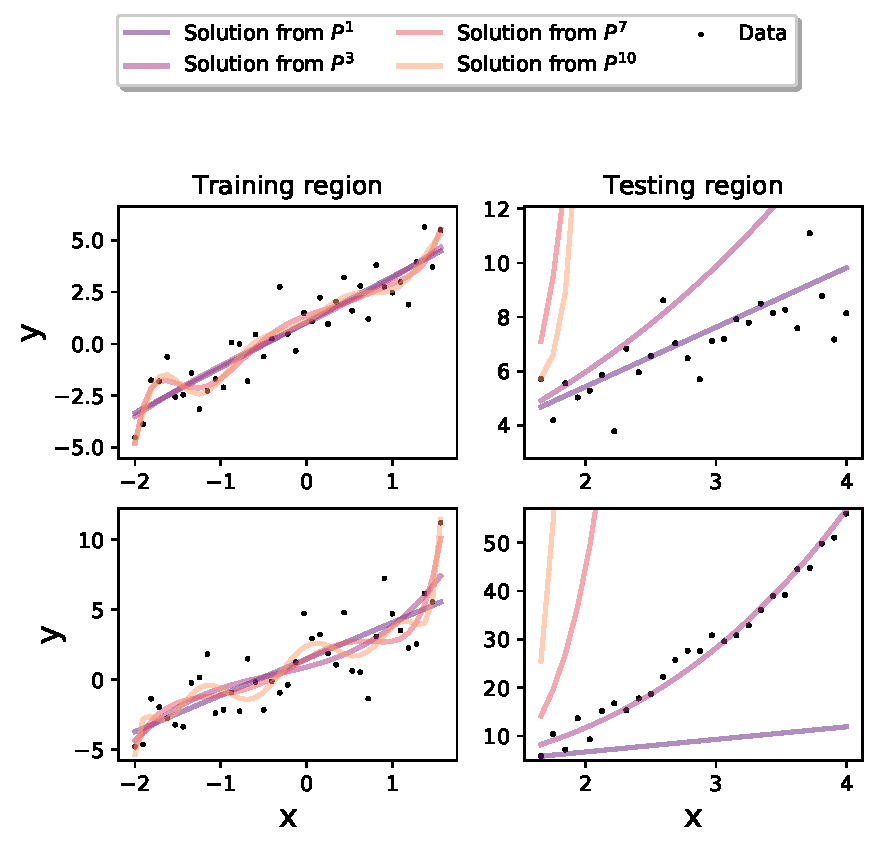
\includegraphics[width=\textwidth]{../figures/y_distr.pdf}
\caption[Illustrating over-fitting with polynomial regression]{Polynomial regression of varying degrees on data drawn from a linear distribution on above and a cubic distribution on the bottom. Models of varying complexity indicated by their basis $P^n$ are fit to the train data and evaluated on the test region, shown in the left and right columns. We observe that the higher order solutions follow what we observe to be  spurious-noise generated features in the data. This is what we call over-fitting. In the bottom column observe that the model with appropriate complexity, $f(x_i) \in P^3$, follows the true trend also in the test region while the linear and higher order models all miss. The linear model does not have the capability to express the complexities of the data and is said to be under-fit. Additionally we observe that the higher order polynomials degrade in performance extremely rapidly outside the training region.}\label{fig:overfit}
\end{figure}

The previous paragraphs contain some important features that we need to keep in mind going forward. We summarize them here for clarity: 
\begin{itemize}
\item "Fitting is not predicting" (\cite{Mehta2019}). There is a fundamental difference between fitting a model to data and making predictions from unseen samples. \\
\item Generalization is hard. Making predictions in regions of data not seen during training is very difficult, making the importance of sampling from the entire space during training that much more vital. \\
\item Complex models often lead to overfitting. While usually resulting in better results during training in the cases where data is noisy or scarce, predictions are poor outside the training sample. 
\end{itemize}


